%\documentclass[first,firstsupp,handout,compress,notes,navigation]{ETHclass} 
%\documentclass[first,firstsupp,handout,notes]{ETHclass} 
%\documentclass[first,firstsupp,handout]{ETHclass} 
%\documentclass[first,firstsupp,notes]{ETHclass} 
\documentclass[first,firstsupp]{ETHclass}
\usepackage[]{amsmath}
\usepackage{etex}
\usepackage[detect-all]{siunitx}
\usepackage{textcomp}
\usepackage{booktabs}

% Options for beamer:
%
% 9,10,11,12,13,14,17pt  Fontsizes
% 
% compress: navigation bar becomes smaller
% t       : place contents of frames on top (alternative: b,c)
% handout : handoutversion
% notes   : show notes
% notes=onlyslideswithnotes
%
%hyperref={bookmarksopen,bookmarksnumbered} : Needed for menues in
%                                             acrobat. Also need
%                                             pdftex as option or 
%                                             compile with
% pdflatex '\PassOptionsToPackage{pdftex,bookmarksopen,bookmarksnumbered}{hyperref} \input{file}'

%\usepackage{beamerseminar}
%\usepackage[accumulated]{beamerseminar}
                                % remove ``accumulated'' option
                                % for original behaviour
\usepackage{beamerbasenotes}
%\setbeamertemplate{note page}[plain] 
%\setbeameroption{notes on second screen}


\usepackage[pdf]{pstricks}


%\setbeamertemplate{note page}[plain] 
\setbeamertemplate{note page}{\ \\[.3cm]
    \textbf{\color{blue}Notes:}\\%[0.1cm]
    {\footnotesize %\tiny
    \insertnote}}
%\setbeameroption{notes on second screen}

    \usepackage{multimedia}

    \setbeamertemplate{navigation symbols}{} % suppresses all navigation symbols:
% \setbeamertemplate{navigation symbols}[horizontal] % Organizes the navigation symbols horizontally.
% \setbeamertemplate{navigation symbols}[vertical] % Organizes the navigation symbols vertically.
% \setbeamertemplate{navigation symbols}[only frame symbol] % Shows only the navigational symbol for navigating frames.

    \setlayoutscale{0.5}
    \setparametertextfont{\scriptsize}
    \setlabelfont{\scriptsize}

    \DeclareSIUnit[number-unit-product = \,]{\permille}{\textperthousand}
    \newcommand{\energy}{\mathcal{E}}
    \newcommand{\vcenteredinclude}[2]{\begingroup
        \setbox0=\hbox{\includegraphics[#1]{#2}}%
        \parbox{\wd0}{\box0}\endgroup}

        \begin{document}

        \title[Second progress report]{Phase contrast imaging at 100 keV}
        \author{\emph{Matteo Abis}\inst{a} \and %
        Thomas Th\"uring\inst{a} \and %
        Marco Stampanoni\inst{a}}
        \institute[ETHZ and PSI]{\inst{a} ETH Z\"urich and Paul Scherrer
    Institut}
    \renewcommand{\today}{28th May 2013}
    \setcounter{framenumber}{0}
    \begin{frame}
        \maketitle
    \end{frame}
    \setcounter{framenumber}{1}
    \begin{frame}
        \frametitle{Phase contrast imaging at \SI{100}{\kilo\electronvolt}}
        \tableofcontents
    \end{frame}
    \section{The edge-on setup}
    \setcounter{framenumber}{1}
    \begin{frame}
        \frametitle{The one-dimensional setup at \SI{100}{\kilo\electronvolt}}
        Top view
        \begin{figure}[h]
            \centering
            \includegraphics[width=\textwidth]{setup.pdf}
        \end{figure}
    \end{frame}

    \begin{frame}
        \frametitle{The one-dimensional setup at
            \SI{100}{\kilo\electronvolt}}
        \begin{figure}[h]
            \centering
            \includegraphics[width=.6\textwidth]{setup.pdf}
        \end{figure}
        \begin{itemize}
            \item pitch $\SI{2.8}{\micro\metre}$
            \item first Talbot ($p^2/8\lambda$)
            \item mean energy (SpekCalc):
                $\SI{50}{\kilo\electronvolt}$
            \item maximum sample size $\SI{2}{\centi\metre}$
        \end{itemize}
    \end{frame}
%\note{}
    \section{Alignment}
    \begin{frame}
        \frametitle{The alignment}
        \begin{table}
            \centering
            \begin{tabular}{l r r}
                \toprule
                motor & achieved & required \\
                \midrule
                rotation $x$ & \SI{0.05}{\degree} & \SI{0.10}{\degree}\\
                rotation $y$ & \SI{0.05}{\degree} & \SI{0.10}{\degree}\\
                rotation $z$ & \SI{0.003}{\degree} & \SI{0.010}{\degree}\\
                translation $x$ & \SI{5}{\milli\metre} & ? \\
                translation $z$ & \SI{10}{\micro\metre} & \SI{50}{\micro\metre} \\
                \bottomrule
            \end{tabular}
        \end{table}
        Alignment takes one week
    \end{frame}
    \begin{frame}
        \frametitle{An additional degree of freedom: curvature}
            The right end of G1 in the picture goes up by
        $\SI{50}{\micro\metre}$ on $\SI{3}{\centi\metre}$
        \begin{figure}[h]
            \centering
            \includegraphics[height=0.5\textheight]{bentG1.pdf}
        \end{figure}
        New holders from Gordan keep the gratings flat
    \end{frame}
    \section{Visibility}
    \begin{frame}
        \frametitle{Visibility map}
        working now reliably at $5.0 \pm \SI{0.2}{\percent}$
        \begin{figure}[h]
            \centering
            \includegraphics[height=.65\textheight]{visibility_latest.pdf}
        \end{figure}
    \end{frame}
    \section{Phase drift}
    \begin{frame}
        \frametitle{Strong drift}
        after twenty scans ($\sim\SI{10}{\minute}$)
        \begin{figure}[h]
            \centering
            \includegraphics[height=.65\textheight]{drift_pixels.pdf}
        \end{figure}
    \end{frame}
    \begin{frame}
        \frametitle{Drift correction}
        linear fit $\rightarrow$ subtraction
        \begin{figure}[h]
            \centering
            \includegraphics[height=.65\textheight]{drift_fit.pdf}
        \end{figure}
    \end{frame}
    \section{The first images}
    \begin{frame}
        \frametitle{The first noisy image}
        Head of a metal screw
        \begin{figure}[h]
            \centering
            \includegraphics[height=.65\textheight]{2013_04_16_screw.pdf}
        \end{figure}
    \end{frame}
    \begin{frame}
        \frametitle{Increasing the exposure time}
        \SI{14}{\hour} scan: $25$ steps $\times \SI{15}{\second} \times
        100$\\
        field of view $2.5\times\SI{1}{\centi\metre}$
        \begin{figure}[h]
            \centering
            \includegraphics[height=.6\textheight]{2013_05_16_screw.pdf}
        \end{figure}
    \end{frame}
    \begin{frame}
        \frametitle{Increasing the exposure time}
        \SI{14}{\hour} scan: $25$ steps $\times \SI{15}{\second} \times
        100$\\
        field of view $2.5\times\SI{1}{\centi\metre}$
        \begin{figure}[h]
            \centering
            \includegraphics[height=.6\textheight]{chip-rot.pdf}
        \end{figure}
    \end{frame}
    \begin{frame}
        \frametitle{Increasing the exposure time}
        \SI{14}{\hour} scan: $25$ steps $\times \SI{15}{\second} \times
        100$\\
        field of view $2.5\times\SI{1}{\centi\metre}$
        \begin{figure}[h]
            \centering
            \only<1>{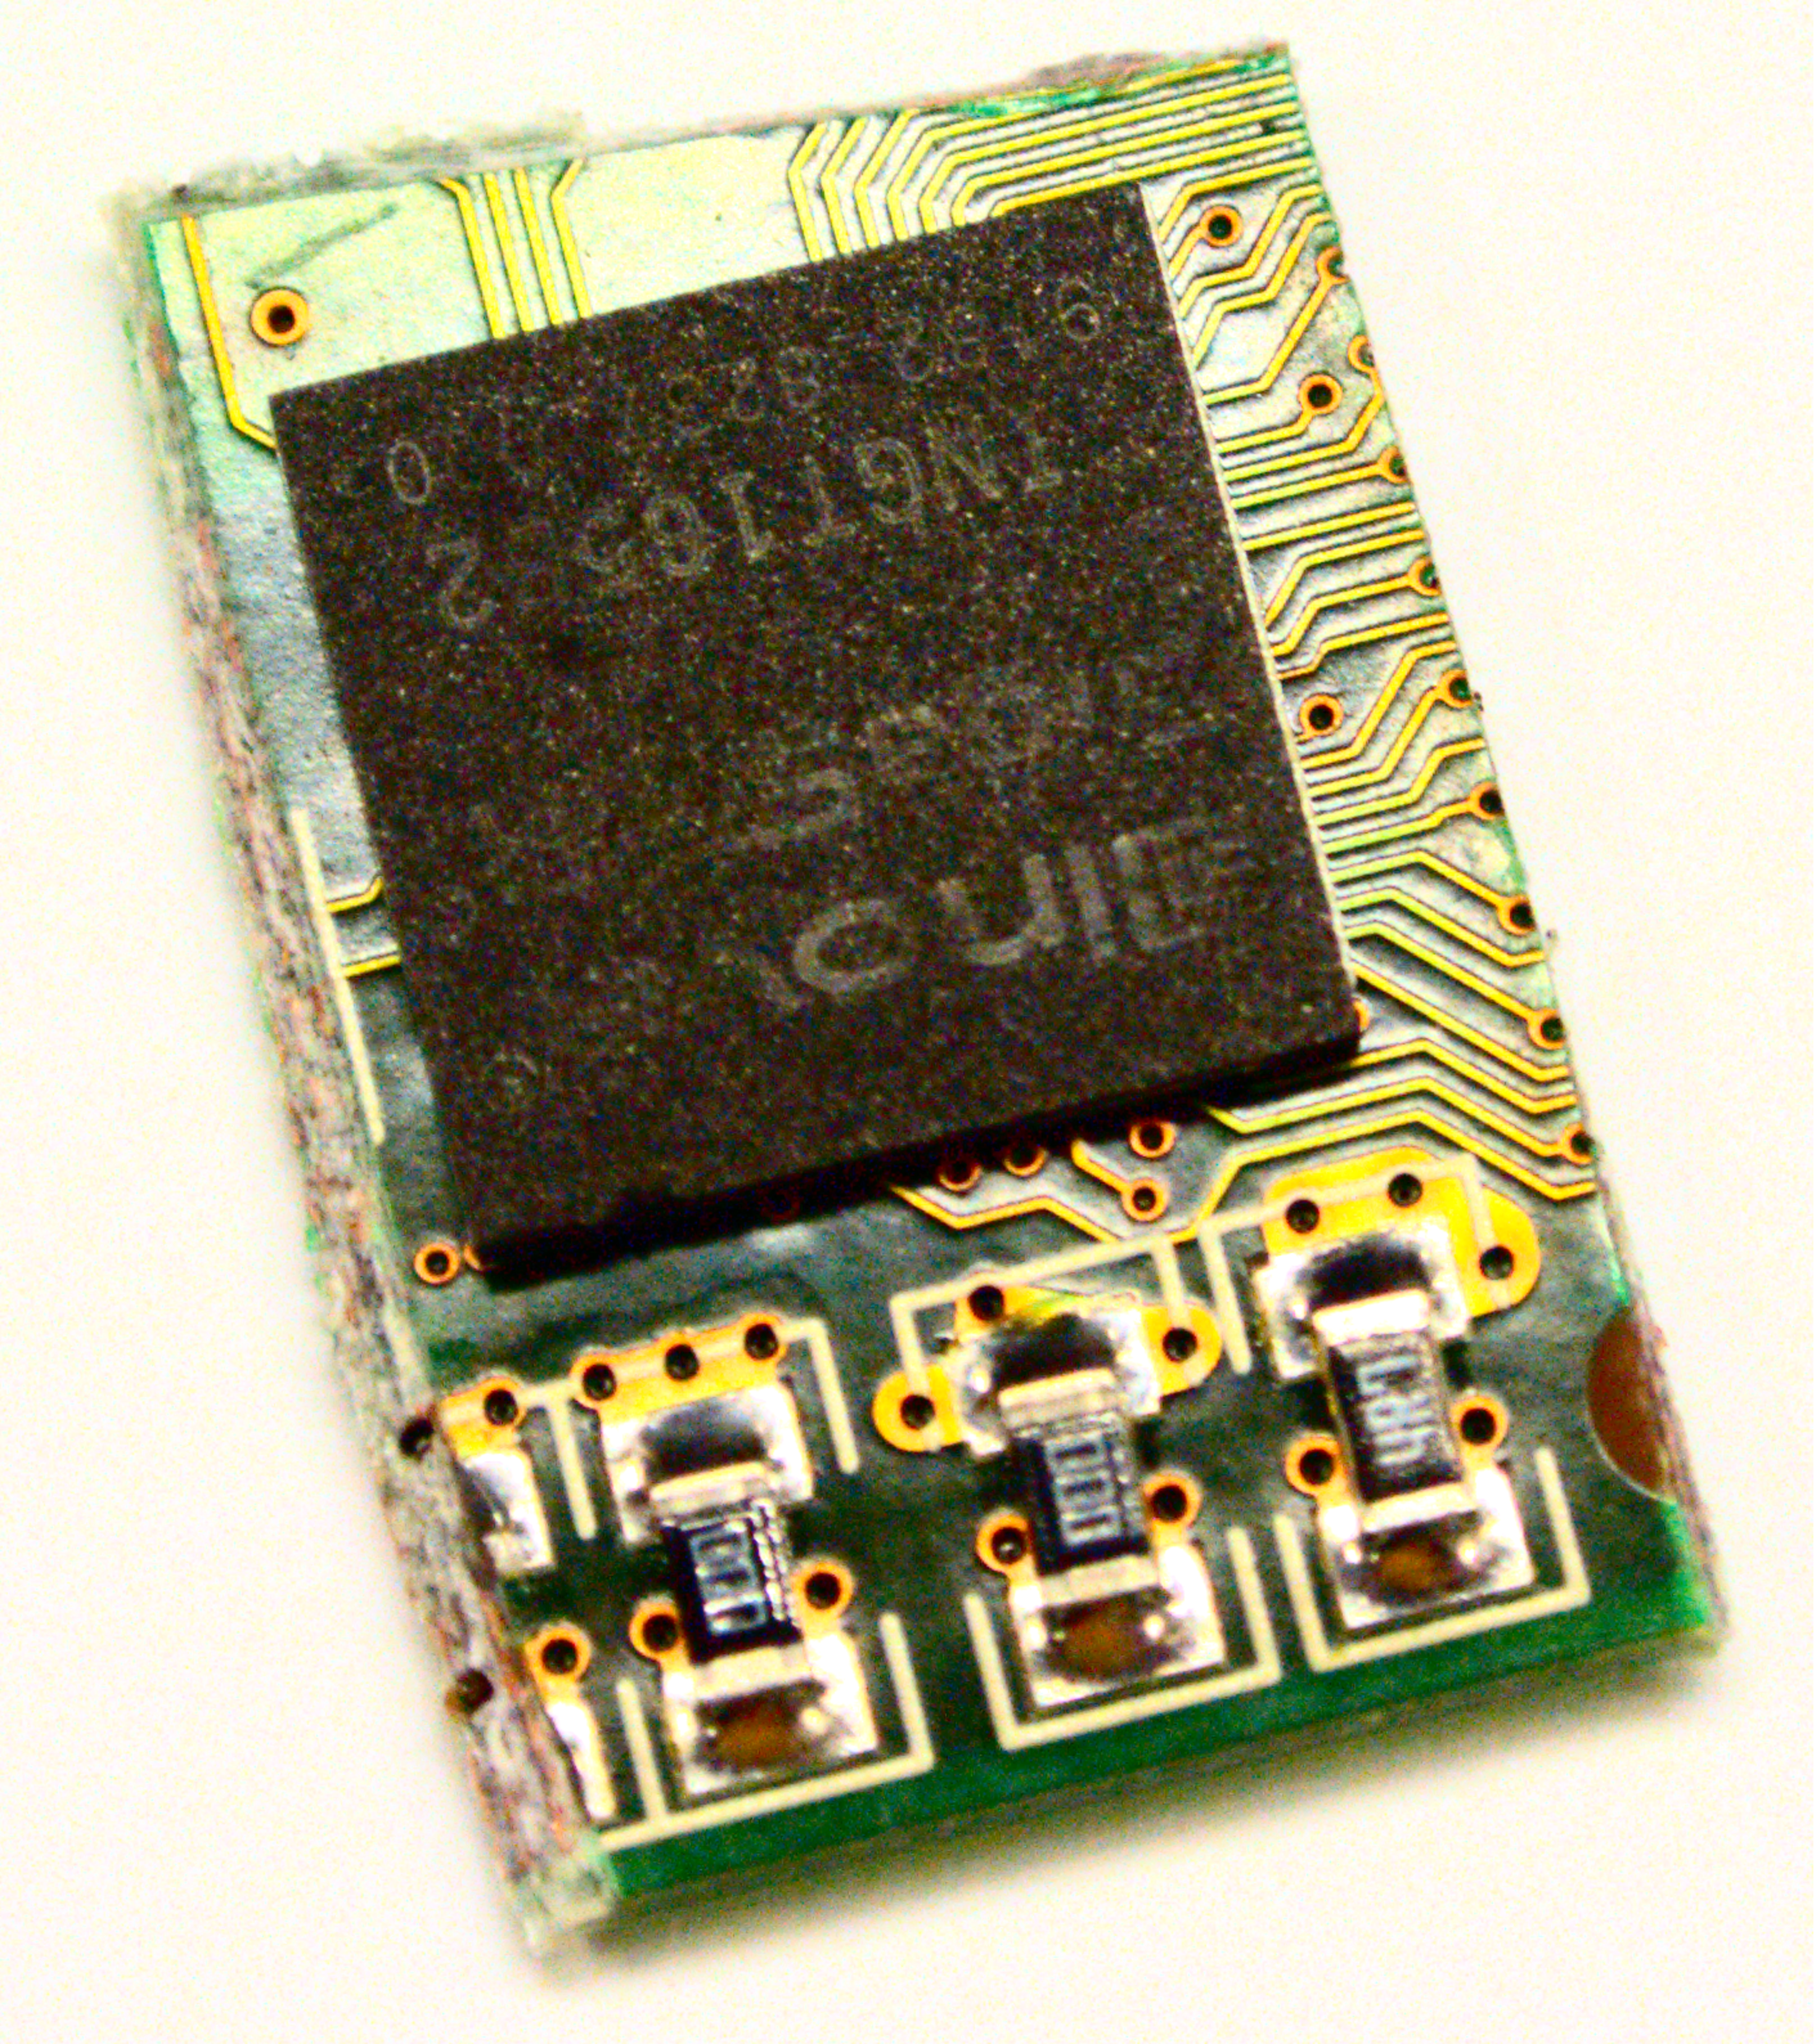
\includegraphics[height=.6\textheight]{chip_overlay_empty.pdf}}
            \only<2>{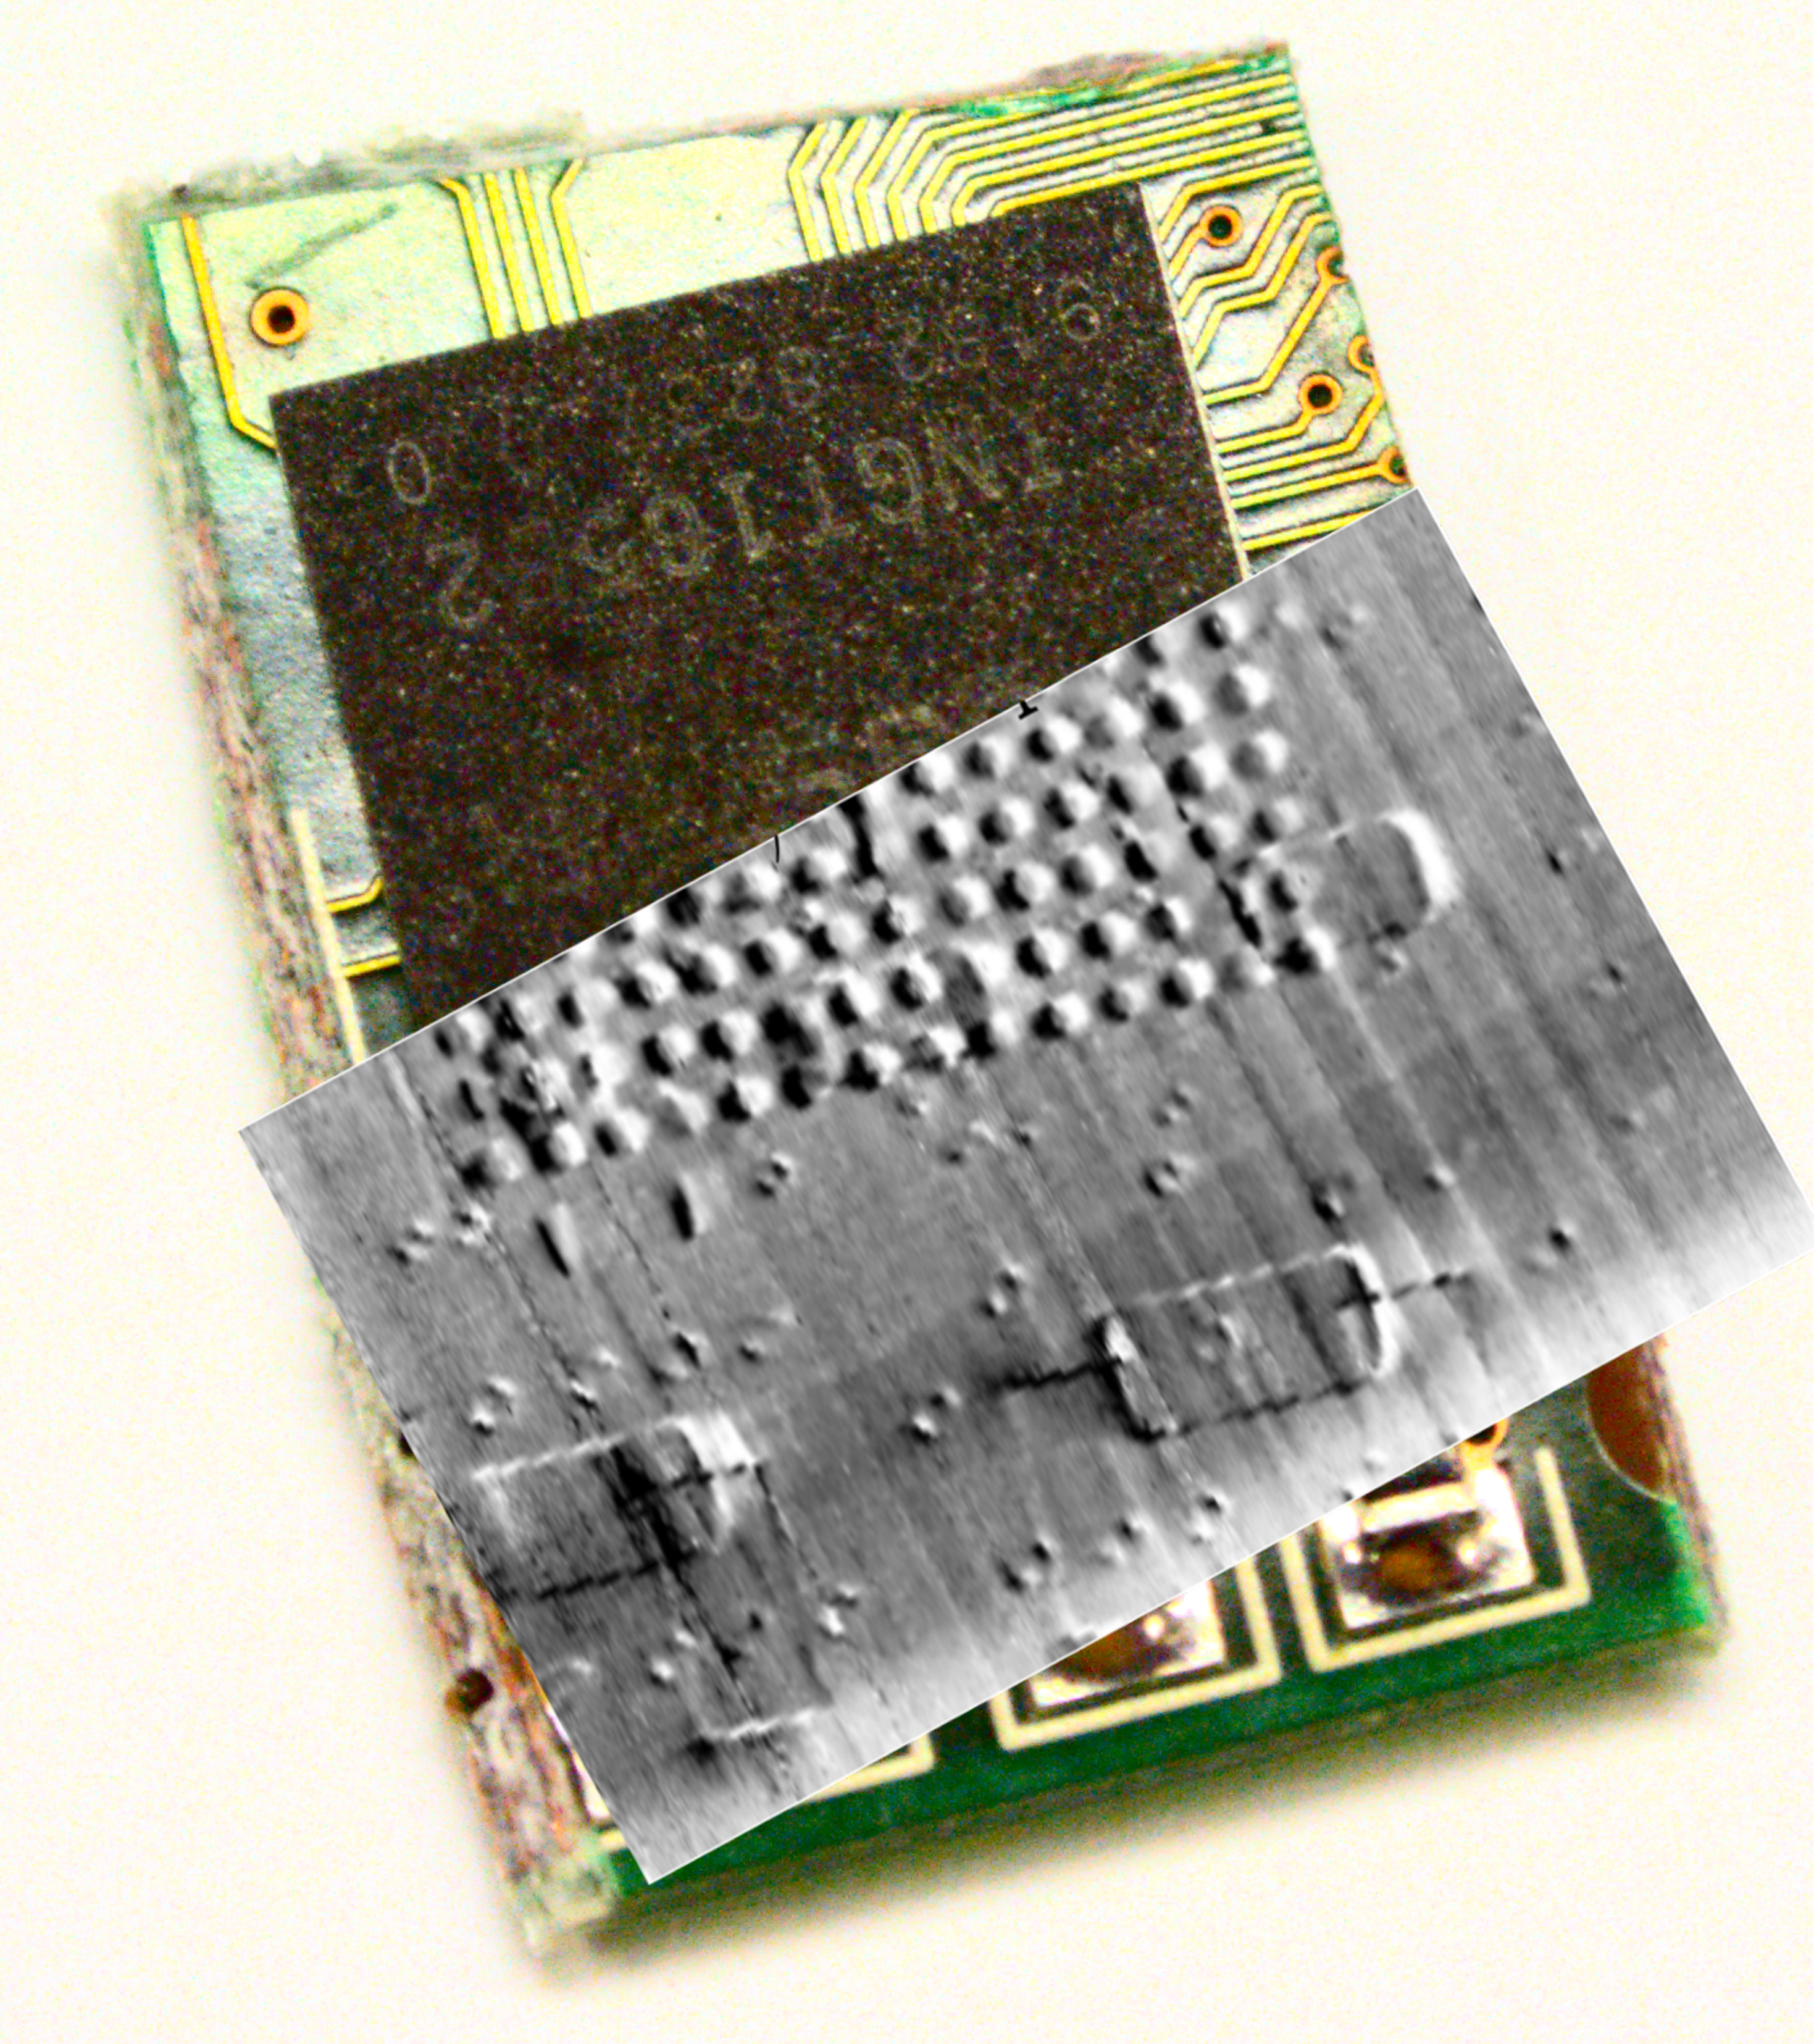
\includegraphics[height=.6\textheight]{chip_overlay_full.pdf}}
        \end{figure}
    \end{frame}
    \begin{frame}
        \frametitle{A biological sample}
        \SI{14}{\hour} scan: $25$ steps $\times \SI{15}{\second} \times
        100$\\
        field of view $2.5\times \SI{1}{\centi\metre}$
        \begin{figure}[h]
            \centering
            \includegraphics[height=.5\textheight]{2013_05_21_toe.pdf}
        \end{figure}
        \alert{energy is too high}
    \end{frame}
    \section{Deep questions ahead}
    \begin{frame}
        \frametitle{Can high-energy phase contrast work?}
        \alert{Pushing grating interferometry towards its physical limits.}
    \end{frame}
    \begin{frame}
        \frametitle{The signal becomes smaller}
        \begin{equation*}
            \varphi = \frac{\lambda d}{p_2} \frac{\partial \Phi}{\partial y}
            \propto \mathcal{E}^{-2}
        \end{equation*}
        Possible solutions:
        \begin{itemize}
            \item other samples \only<2>{$\longrightarrow$ \alert{is biological imaging
                possible?}}
            \item larger distances \only<2>{$\longrightarrow$
                    \alert{polychromaticity and flux}}
            \item smaller pitches  \only<2>{$\longrightarrow$
                    \alert{even more difficult fabrication}} 
        \end{itemize}
    \end{frame}
    \begin{frame}
        \frametitle{The noise becomes larger}
        \begin{equation*}
            \sigma_\varphi \propto \frac{1}{v\sqrt{N}}
        \end{equation*}
        \begin{itemize}
            \item difficult fabrication of the gratings $\rightarrow$ low visibility
            \item low detection efficiency
            \item little room for filtering
        \end{itemize}
    \end{frame}
    \begin{frame}
        \frametitle{What is a high-energy absorption image?}
        \begin{figure}[h]
            \centering
            \includegraphics[width=.6\textwidth]{carbon_cross_sections}
        \end{figure}
    \end{frame}
    \begin{frame}
        \frametitle{Thanks!}
    \end{frame}
    \end{document}
